%%%%%%%%%%%%%%%%%%%%%%%%%%%%%%%%%%%%%%%%
%12pt: grandezza carattere
%a4paper: formato a4
%openright: apre i capitoli a destra
%twoside: serve per fare un documento fronteretro
%report: stile tesi (oppure book)
\documentclass[12pt,a4paper,openright,twoside]{report}

\usepackage[italian]{babel}
\usepackage[latin1]{inputenc}
\usepackage{fancyhdr}
\usepackage{indentfirst}
\usepackage{graphicx}
\usepackage{newlfont}
%librerie matematiche
\usepackage{amssymb}
\usepackage{amsmath}
\usepackage{latexsym}
\usepackage{amsthm}
\usepackage{listings}
\usepackage{chngcntr}
\usepackage[chapter]{minted}


\oddsidemargin=30pt \evensidemargin=20pt%impostano i margini
\hyphenation{sil-la-ba-zio-ne pa-ren-te-si}

\usepackage[square, numbers, comma, sort&compress]{natbib} %Bibliografia
\usepackage{hyperref}
\usepackage{float}

\usepackage[pass]{geometry}

%comandi per l'impostazione della pagina, vedi il manuale della libreria fancyhdr per ulteriori delucidazioni
\pagestyle{fancy}\addtolength{\headwidth}{20pt}
\renewcommand{\chaptermark}[1]{\markboth{\thechapter.\ #1}{}}
\renewcommand{\sectionmark}[1]{\markright{\thesection \ #1}{}}
\rhead[\fancyplain{}{\bfseries\leftmark}]{\fancyplain{}{\bfseries\thepage}}
\cfoot{}

\linespread{1.3} %comando per impostare l'interlinea

\renewcommand{\listingscaption}{Codice}
\renewcommand{\listoflistingscaption}{Elenco dei Codici}

\begin{document}
%%%%%%%%%%%%%%%%%%%%%%%%%%%%%%%%%%%%%%%%
% FRONTESPIZIO
\newgeometry{hmarginratio=1:1}
\begin{titlepage}
\begin{center}

\includegraphics[width=2.56in]{figures/logo/logo_unibo.png}\\
% {{\Large{\textsc{Alma Mater Studiorum $\cdot$ Universit\`a di
% Bologna}}}} \rule[0.1cm]{14.7cm}{0.1mm}
% \rule[0.5cm]{14.7cm}{0.6mm}
\vspace{5mm}
{\small{\bf SCUOLA DI INGEGNERIA E ARCHITETTURA\\
\vspace{2mm}
Dipartimento di Informatica -- Scienza e Ingegneria\\
\vspace{2mm}
Corso di Laurea in Ingegneria Informatica }}
%se Laurea Magistrale scrivere "Corso di Laurea Magistrale in Ingegneria Informatica"
\end{center}
\vspace{3,8mm}
\begin{center}
{\LARGE{\bf Cybersecurity e finanza:\\
\vspace{3,5mm}
analisi e studio delle conseguenze\\
\vspace{3,5mm}
finanziare degli attacchi informatici\\
\vspace{3,5mm}
sulle aziende\\
\vspace{3,5mm}}}
  
\end{center}
\vspace{9,5mm}
\par
\noindent
\begin{minipage}[t]{0.47\textwidth}
{\normalsize{\bf Relatore:\\
Prof. Dr. Marco Prandini\\

Correlatore:\\
Dr. Alessandro Vannini}}
\end{minipage}
\hfill
\begin{minipage}[t]{0.47\textwidth}\raggedleft
{\normalsize{\bf Presentata da:\\
Leonardo Ciacco}}
\end{minipage}
\vspace{7,5mm} % da aumentare a 10, 20 o 30 se non si inseriscono i correlatori
\begin{center}
{\normalsize{\bf Appello unico\\%inserire il numero dell'appello in cui ci si laurea CAPIRE
Anno Accademico 2024/2025}}%inserire l'anno accademico a cui si è iscritti
\end{center}
\end{titlepage}

\restoregeometry


%%%%%%%%%%%%%%%%%%%%%%%%%%%%%%%%%%%%%%%%
% ABSTRACT 
\clearpage{\pagestyle{empty}\cleardoublepage}
\pagenumbering{roman}
\renewcommand{\abstractname}{Abstract}
\phantomsection
\addcontentsline{toc}{chapter}{Abstract}
\begin{abstract}
    Questo \`e l'abstract: un riassunto dell'introduzione di massimo 300 parole. Da scrivere alla fine.
\end{abstract}


%%%%%%%%%%%%%%%%%%%%%%%%%%%%%%%%%%%%%%%%
% RINGRAZIAMENTI 
\clearpage{\pagestyle{empty}\cleardoublepage}
\chapter*{Ringraziamenti}
\phantomsection
\addcontentsline{toc}{chapter}{Ringraziamenti}
Qui possiamo ringraziare il mondo intero!!!!!!!!!!\\
Ovviamente solo se uno vuole, non \`e obbligatorio.

\clearpage{\pagestyle{empty}\cleardoublepage}



%%%%%%%%%%%%%%%%%%%%%%%%%%%%%%%%%%%%%%%%
% INDICE 
\tableofcontents %crea l'indice
%imposta l'intestazione di pagina
\rhead[\fancyplain{}{\bfseries\leftmark}]{\fancyplain{}{\bfseries\thepage}}
\lhead[\fancyplain{}{\bfseries\thepage}]{\fancyplain{}{\bfseries
Indice}}



%%%%%%%%%%%%%%%%%%%%%%%%%%%%%%%%%%%%%%%%
% ELENCO DELLE FIGURE
\clearpage{\pagestyle{empty}\cleardoublepage}
\renewcommand{\listfigurename}{Elenco delle Figure}
\phantomsection
\addcontentsline{toc}{chapter}{Elenco delle Figure}
\listoffigures %crea l'elenco delle figure



%%%%%%%%%%%%%%%%%%%%%%%%%%%%%%%%%%%%%%%%
% ELENCO DELLE TABELLE
\clearpage{\pagestyle{empty}\cleardoublepage}
\renewcommand{\listtablename}{Elenco delle Tabelle}
\phantomsection
\addcontentsline{toc}{chapter}{Elenco delle Tabelle}
\listoftables %crea l'elenco delle tabelle



%%%%%%%%%%%%%%%%%%%%%%%%%%%%%%%%%%%%%%%%
% INTRODUZIONE
\clearpage{\pagestyle{empty}\cleardoublepage}
\chapter{Introduzione} 
\lhead[\fancyplain{}{\bfseries\thepage}]{\fancyplain{}{\bfseries\rightmark}}
\pagenumbering{arabic} %mette i numeri arabi
Questa \`e l'introduzione: da scrivere alla fine, un breve riassunto su cosa si andr\`a ad affrontare nella tesi.
Le linee guida per la stesura della Tesi di Laurea sono al seguente link \href{https://ulis.se/thesis/}{https://ulis.se/thesis/}.

\section{Prima Sezione} %crea la sezione
Questa \`e la prima sezione.


Ora vediamo un elenco numerato: %crea un elenco numerato
\begin{enumerate}
\item primo oggetto
\item secondo oggetto
\item terzo oggetto
\item quarto oggetto
\end{enumerate}

\begin{figure}[h] %crea l'ambiente figura; [h] sta per here, cioè la figura va qui
\begin{center} %centra nel mezzo della pagina la figura \includegraphics[width=5cm]{figura.eps} inserisce una figura larga 5cm se si vuole usare va scommentata

%inserisce la legenda ed etichetta la figura con \label{fig:prima}
\caption[legenda elenco figure]{legenda sotto la figura}\label{fig:prima}
\end{center}
\end{figure}


\section{Seconda Sezione}
Ora vediamo un elenco puntato:
\begin{itemize} %crea un elenco puntato
\item primo oggetto
\item secondo oggetto
\end{itemize}


\section{Altra Sezione}
Vediamo un elenco descrittivo:

\begin{description} %crea un elenco descrittivo
  \item[OGGETTO1] prima descrizione;
  \item[OGGETTO2] seconda descrizione;
  \item[OGGETTO3] terza descrizione.
\end{description}


\subsection{Altra SottoSezione}
%crea una sottosottosezione

\subsubsection{SottoSottoSezione}Questa sottosottosezione non viene
numerata, ma \`e solo scritta in grassetto.


\section{Altra Sezione} %crea una sottosezione
Vediamo la creazione di una tabella; la tabella \ref{tab:uno}
(richiamo il nome della tabella utilizzando la label che ho messo sotto):
la facciamo di tre righe e tre colonne, la prima colonna
``incolonnata'' a destra (r) e le altre centrate (c):\\
\begin{table}[h] %ambiente tabella (serve per avere la legenda)
\begin{center} %centra nella pagina la tabella
\begin{tabular}{r|c|c} %tre colonne con righe verticali prodotte con |
\hline \hline                           %inserisce due righe orizzontali
$(1,1)$ & $(1,2)$ & $(1,3)$\\ %& separa le colonne e con
\hline                                  %inserisce una riga orizzontale
$(2,1)$ & $(2,2)$ & $(2,3)$\\ %  \\ va a capo
\hline                                  %inserisce una riga orizzontale
$(3,1)$ & $(3,2)$ & $(3,3)$\\
\hline \hline                           %inserisce due righe orizzontali
\end{tabular}
\caption[legenda elenco tabelle]{legenda tabella}\label{tab:uno}
\end{center}
\end{table}


\section{Altra Sezione}\label{sec:prova}%posso mettere le label anche alle section
In questa sezione voglio fare un riferimento alla bibliografia: questo \`e il mio riferimento 
prova cit \cite{enisa_threat_landscape}

\subsection{Listati dei programmi}
\subsubsection{Primo Listato}
\begin{verbatim}
        In questo ambiente     posso scrivere      come voglio,
lasciare gli spazi che voglio e non % commentare quando voglio
e ci sarà scritto tutto.
Quando lo uso è meglio che disattivi il Wrap del WinEdt
\end{verbatim}
\clearpage{\pagestyle{empty}\cleardoublepage}



%%%%%%%%%%%%%%%%%%%%%%%%%%%%%%%%%%%%%%%%
% STATO DELL'ARTE
\chapter{Analisi dello stato dell'arte e del contesto}
Il presente capitolo mira a fornire le informazioni fondamentali, necessarie a comprendere i futuri sviluppi. A questo scopo sono definiti alcuni concetti chiave in ambito di sicurezza informatica:
\begin{itemize}
    \item rischio
    \item sicurezza
    \item minaccia
    \item vulnerabilit\`a
    \item attacco
\end{itemize}
Con \textbf{rischio} si intende la possibilit\`a che azioni umane o eventi  abbiano un impatto su ci\`o a cui \`e attribuito valore. \`E quindi corretto affermare che si tratta di una grandezza, e come tale \`e quantificabile, \`e infatti direttamente proporzionale alla probabilit\`a di avvenimento e all'impatto che avrebbe sui beni colpiti. La valutazione del rischio, mirata alla sua gestione e controllo, parte dalla stima quanto pi\`u accurata di queste due variabili.\\
\\
La \textbf{sicurezza} \`e il processo di contenimento del rischio che consiste essenzialmente nella cura di tre propriet\`a fondamentali: riservatezza (inaccessibilit\`a delle informazioni a chi non ha il permesso di consultarle), integrit\`a (garanzia di correttezza delle informazioni) e disponibilit\`a(possibilit\`a di accesso e utilizzo delle informazioni e i servizi offerti).\\
\\
La \textbf{minaccia} consiste nella potenziale compromissione di una o pi\`u delle propriet\`a sopracitate, e, da concetto astratto, si concretizza in un \textbf{attacco}: azione di sfruttamnento (\textit{exploit}) delle vulnerabilit\`a di un sistema\\

\section{Tipologie di attacco}
ENISA (Agenzia dell'Unione europea per la cibersicurezza) raggruppa gli attacchi informatici in otto categorie principali.\cite{enisa_threat_landscape}
\subsection{Ransomware}
Definito come un tipo d attacco in cui gli attori coinvolti prendono il controllo di un bene del bersaglio e chiedono un riscatto (in inglese \textit{ransom}) in cambio della restituzione. \`E un tipo di attacco fatto generalmente per scopi economici, ma, essendo anche uno dei pi\`u diffusi evolve rapidamente, sia dal punto di vista delle tecniche di estorsione che degli obiettivi.\\

\subsection{Malware}
Si tratta di un termine ombrello, descrive tutti i software o firmware con lo scopo di eseguire un processo non autorizzato sulla macchina ospitante il cui risultato \`e la compromissione di una delle tre propiet\`a della sicurezza.\\
\subsection{Ingegneria sociale}
Gli attacchi tramite ingegneria sociale si distinguono per lo sfruttamento della vulnerabilit\`a derivata dall'errore umano. Consinstono nel mettere in atto tecniche di manipolazione per indurre chi coinvolto nella gestione dei beni bersaglio a rilasciare informazioni sensibili, concedere permessi 
apparentemente innocui, visitare siti, aprire file, documenti o e-mails con contenuto malevolo. Un esempio pu\`o essere il \textit{phishing}, attacco in cui si cerca di indurre la vittima ad aprire un link ad un sito che scarica un malware.\\
L'ingegneria sociale \`e spesso protagonista delle fasi iniziali di un attacco, ma questo non esclude che possa essere impiegata in stadi pi\`u avanzati. Ad esempio, \`e chiamata BEC (\textit{Business E-mail Compromise}) l'intrusione tramite vecchie credenziali aziendali che le sfrutta, fingendosi parte dell'organizzazione, per ottenere dagli ex colleghi informazioni, denaro, o risorse altrimenti inaccessibili.\cite{IBM_BEC}\\

\subsection{Violazioni di dati}
Tecnicamente vi ci si riferisce con i termini inglesi \textit{data breach} o \textit{data leak}.  
Da definizione del GDPR, per violazione dei dati personaliintendiamo la "violazione di sicurezza che comporta accidentalmente o in modo illecito la distruzione, la perdita, la modifica, la divulgazione non autorizzata o l'accesso ai dati personali trasmessi, conservati o comunque trattati" (articolo 4.12 GDPR). \\
La differenza risiede nell'intenzionalità: il \textit{breach} \`e un attacco con l'esplicito obiettivo di ottenere o diffondere dati sensibili o protetti, il \textit{leak} è originato da un errore che porta ad una indesiderata perdita o messa a disposizione di dati sensibili. \\

\subsection{Minacce alla disponibilit\`a: DoS}
Per definizione, un DDoS (\textit{Distriubuted Denial of Service}), si verifica come risultato di un attacco che mira a rendere inaccessibili servizi o risorse tramite, per esempio, uno sproporzioato volume di richieste che sovraccarica i componenti della struttura attaccata.
In questo caso quindi l'obiettivo risiede nella semplice interruzione dei servizi erogati.\\

\subsection{Minacce alla disponibilit\`a: minacce ad Internet}
Alla base della disponibilit\`a dei servizi nella societ\`a dell'informazione vi \`e l'infraastruttura di internet, che se subisce guasti distribuiti pu\`o comprometterne quasi completamente l'erogazione. Sebbene sia un'ipotesi remota,  blackout, disastri naturali, interruzione forzata da parte del governo o attacchi su larga scala rappresentano una minaccia concreta che non pu\`o essere sottovalutata.\\

\subsection{Manipolazione delle informazioni}
Si chiama \textit{Foreign Information Manipulation and Interference}, abbreviato in FIMI, l'insieme di strategie di manipolazione dell'opinione pubblica da parte di enti, governativi e non, volte ad inserirsi nel dibattito in maniera massiccia e organizzata. Ci\`o mina i processi decisionali democratici tramite campagne di disinformazione e narrazioni precostruite.\\
\subsection{Attacchi alla catena di fornituta}
Pi\`u comunemente  chiamati \textit{supply chain attacks}, sono attacchi che sfruttano la fiducia riposta nei servizi offerti da partner commerciali o fornitori, colpendo l'obiettivo indirettamente tramite la compromissione di un fornitore legittimo.\\
Pi\`u formalmente, un attacco \`e considerato in parte di natura \textit{supply chain} se consiste nella combinazione di almeno due attacchi coordinati. Perch\'e sia identificato come tale, devono infatti essere bersaglio sia l'obiettivo intermedio, fornitore, che l'obiettivo finale, naturalmente vulnerabile nei confronti chi valuta fonte sicura. \\
%SolarWinds
%was one of the first revelations of this kind of attack and showed the potential impact of supply chain attacks. It was observed that threat actors are continuing to feed on this source to conduct their operations and gain a
%foothold within organisations, to benefit from the widespread impact and large victim base of such attacks



\section{Contesto economico}
Con l'esponenziale crescita ed espansione dei mezzi di informazione, crescono anche i mercati illeciti, precisamente il costo del cybercrimine era di \$3 trilioni nel 2015 e, si stima, toccher\`a i \$10.5 trilioni durante il 2025\cite{cybercrime_magazine}. Se fosse il PIL di uno stato sarebbe sicuramente tr i primi cinque al mondo.\\
In un paorama di questo tipo le aziende quotate in borsa, soprattutto le pi\`u in risalto come quelle in indici come S\&P500, sono un bersaglio estremamente appetibile per chiunque abbia i mezzi e l'intenzione di danneggiarle in quanto:
\begin{itemize}
  \setlength{\itemsep}{0pt}
  \setlength{\parskip}{0pt}       
  \renewcommand{\labelitemi}{\textbf{--}} 
  \item sono in possesso di grandi quantit\`a di \textbf{dati sensibili}: questo sopratutto se si tratta di grandi aziende o se specializzate nel settore, ma chiaramente, se l'obiettivo \`e il furto di informazioni, un'alta concentrazione delle stesse agisce da incentivo;
  \item sono facilmente \textbf{valutabili}: per eseguire un attacco \textit{ransomware} occorre anche commisurare la richiesta di riscatto al valore del bene per l'azienda e alla sua disponibilit\`a economica, i bilanci pubblici offrono qundi una fonte di informazioni  preziosa;
  \item se attaccate, hanno \textbf{reazioni} spesso \textbf{prevedibili}: secondo un rapporto di Accenture del 2010 \cite{accenture2010}, le aziende che subiscono un attacco sperimentano un calo di prezzo delle azioni che si aggira solitmente intorno al 5\%, rivelando come l'attacco potrebbe essere sfruttato ulteriormente come strumento di controllo illecito del mercato per trarre  ulteriori profitti collaterali.
\end{itemize}
Solo nel 2023, il 21\% selle aziende in S\&P500 hanno subito un \textit{breach}\cite{SecurityScorecard_SP500}.\\
Inoltre, i danni connessi agli attacchi sono ugualmente preoccupanti, tra questi:
\begin{itemize}
  \setlength{\itemsep}{0pt}   
  \setlength{\parskip}{0pt}       
  \renewcommand{\labelitemi}{\textbf{--}}  
  \item ripercussioni legali;
  \item perdita di fiducia di clienti ed investitori.
\end{itemize}

\section{Metodologia}
Lo studio si propone di analizzare 15 casi di attacchi informatici, con focus sulle ripercussioni che questi hanno avuto sull'azienda.\\
Gli attacchi sono di vario tipo, e sono avvenuti tra il 2011 e il 2024 l'analisi \`e condotta con l'obiettivo di individuare un trend e in generale valutare la minacci crescente del cybercrimine.\\  
\clearpage{\pagestyle{empty}\cleardoublepage}



%%%%%%%%%%%%%%%%%%%%%%%%%%%%%%%%%%%%%%%%
% Attacchi e conseguenze finanziarie
\chapter{Attacchi e conseguenze finanziarie}
Nota: la maggior parte dei grafici proviene da \href{https://www.macrotrends.net/}.
\section{Epsilon data breach (2011)}
\subsection{Descrizione}

\subsection{Impatto diretto}

\subsection{Impatto indiretto}

\subsection{Note}
\section{Sony Playstation Network (2011)}
\subsection{Descrizione}
Sony dichiar\`o che tra il 17 e il 19 aprile 2011 avvene un importante \textit{data breach} , a seguito di cui disabilit\`o per una settimana il servizio online Playstation Network. L'attacco port\`o al furto di dati sensibili riguardanti 77 milioi di account\cite{Sony_PNT_guardian}\cite{Sony_pnt}.\\
\subsection{Impatto diretto}
Sony sub\`i diverse conseguenze legali, che unite agli obblighi di miglioramento della sicurezza, si stima ebbero un costo complessivo di \$171 milioni.\\
\subsection{Impatto indiretto}
Come si pu\`ovedere dalla figura ... e nelle fonti \cite{Sony_pnt} la compagnia sub\`i, nei primi giorni, un calo del valore delle azioni ben superiore al 3\%.\\

\begin{figure}[h] 
\begin{center} 
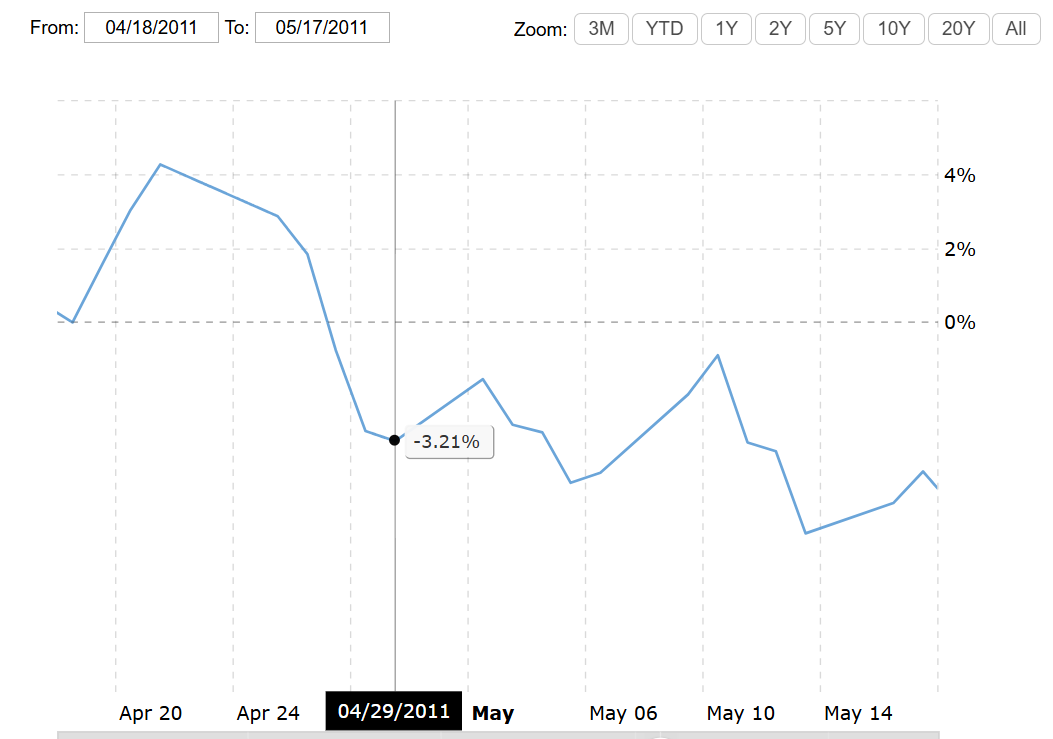
\includegraphics[width=10cm]{figures/sony_2011_shortTerm.png} 
\caption[Grafico Sony PSN short]{Impatto a breve termine Sony Playstation Network Outage}\label{fig:pnt1}
\end{center}
\end{figure}

A seguito inizia un periodo di contrazione che, possiamo osservare, porta i valori delle azioni da pi\`u di \$5 nel periodo antecedente alla crisi, fino a scendere sotto i \$2 nel 2013 (adjusted). Associare la parabola discendente esclusivamente all'attacco \`e forse esagerato, \`e sicuramente un fattore rilenvante.\\ 

\begin{figure}[h] 
\begin{center} 
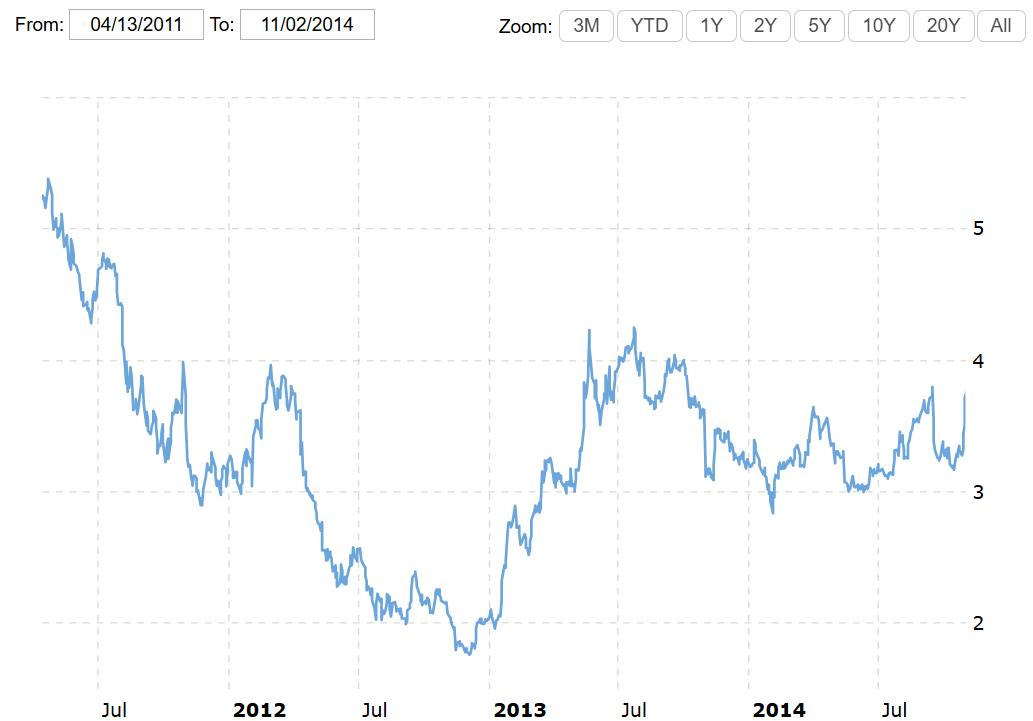
\includegraphics[width=10cm]{figures/sony_2011_longTerm.png} 
\caption[Grafico Sony PSN short]{Impatto a lungo termine Sony Playstation Network Outage}\label{fig:pnt2}
\end{center}
\end{figure}


\subsection{Note}
Le comunicazioni furono tardive e poco precise, gli azionisti ebbero notizia del motivo per cui Playstation Network era disabilitato solo 7 giorni dopo, e i comunicati ai clienti non furono da meno, alimentando malcontento e sfiducia nelle capacit\`a dell'azienda\cite{Sony_pnt}.
\section{Target (2013)}
\subsection{Descrizione}

\subsection{Impatto diretto}

\subsection{Impatto indiretto}

\subsection{Note}
\section{Sony Pictures (2014)}
\subsection{Descrizione}

\subsection{Impatto diretto}

\subsection{Impatto indiretto}

\subsection{Note}
\section{Yahoo (2014)}
\subsection{Descrizione}

\subsection{Impatto diretto}

\subsection{Impatto indiretto}

\subsection{Note}
\section{Uber (2016, 2022)}
\subsection{Descrizione}

\subsection{Impatto diretto}

\subsection{Impatto indiretto}

\subsection{Note}
\section{FedEx - NotPetya (2017)}
\subsection{Descrizione}

\subsection{Impatto diretto}

\subsection{Impatto indiretto}

\subsection{Note}
\section{Equifax (2017)}
\subsection{Descrizione}

\subsection{Impatto diretto}

\subsection{Impatto indiretto}

\subsection{Note}
\section{British Airways (2018)}
\subsection{Descrizione}

\subsection{Impatto diretto}

\subsection{Impatto indiretto}

\subsection{Note}
\section{Marriot International (2018)}
\subsection{Descrizione}

\subsection{Impatto diretto}

\subsection{Impatto indiretto}

\subsection{Note}
\section{Capital One (2019)}
\subsection{Descrizione}

\subsection{Impatto diretto}

\subsection{Impatto indiretto}

\subsection{Note}
\section{SolarWinds (2020)}
\subsection{Descrizione}

\subsection{Impatto diretto}

\subsection{Impatto indiretto}

\subsection{Note}
\section{Colonial Pipeline (2021)}
\subsection{Descrizione}

\subsection{Impatto diretto}

\subsection{Impatto indiretto}

\subsection{Note}
\section{MGM Resorts (2023)}
\subsection{Descrizione}

\subsection{Impatto diretto}

\subsection{Impatto indiretto}

\subsection{Note}
\section{Change Healthcare (2024)}
\subsection{Descrizione}

\subsection{Impatto diretto}

\subsection{Impatto indiretto}

\subsection{Note}

\clearpage{\pagestyle{empty}\cleardoublepage}



%%%%%%%%%%%%%%%%%%%%%%%%%%%%%%%%%%%%%%%%
% Analisi dettagliata del precedente capitolo 
\chapter{Analisi dettagliata del precedente capitolo}
Questo sar\`a il capitolo pi\`u importante dove individua trend sugli attacchi e sulle conseguenze.\\
\\href{https://www.overleaf.com/learn/latex/Code\_listing}{listing}.


\clearpage{\pagestyle{empty}\cleardoublepage}



%%%%%%%%%%%%%%%%%%%%%%%%%%%%%%%%%%%%%%%%
% CONCLUSIONI
\chapter{Conclusioni}

Da scrivere alla fine, un breve riassunto di cosa si \`e affrontato, i risultati (se quanto indicato nell'introduzione come obiettivo \`e stato raggiunto) e come \`e possibile continuare la tesi (p.e. se qualcosa non \`e stato affrontato per motivi di tempo o limitazioni hardware).



\clearpage{\pagestyle{empty}\cleardoublepage}



%%%%%%%%%%%%%%%%%%%%%%%%%%%%%%%%%%%%%%%%%%
% RIMUOVERE LE APPENDICI SE NON UTILIZZATE
%imposta l'intestazione di pagina
\renewcommand{\chaptermark}[1]{\markright{\thechapter \ #1}{}}
\lhead[\fancyplain{}{\bfseries\thepage}]{\fancyplain{}{\bfseries\rightmark}}
\appendix %imposta le appendici
\chapter{Prima Appendice} %crea l'appendice
In questa Appendice non si \`e utilizzato il comando:\\
%\verb"" è equivalente all' ambiente verbatim,  ma si utilizza all'interno di un discorso.
\verb"\clearpage{\pagestyle{empty}\cleardoublepage}", ed infatti l'ultima pagina 8 ha l'intestazione con il numero di pagina in alto.
%imposta l'intestazione di pagina
\rhead[\fancyplain{}{\bfseries \thechapter \:Prima Appendice}]
{\fancyplain{}{\bfseries\thepage}}



\clearpage{\pagestyle{empty}\cleardoublepage}



\chapter{Seconda Appendice}
\rhead[\fancyplain{}{\bfseries \thechapter \:Seconda Appendice}]
{\fancyplain{}{\bfseries\thepage}}


\clearpage{\pagestyle{empty}\cleardoublepage}
%%%%%%%%%%%%%%%%%%%%%%%%%%%%%%%%%%%%%%%%%
% BIBLIOGRAFIA
\addcontentsline{toc}{chapter}{Bibliografia}
\label{Bibliography}
\bibliographystyle{IEEEtran}
\bibliography{src/bibliography}
\rhead[\fancyplain{}{\bfseries Bibliografia}]
{\fancyplain{}{\bfseries\thepage}}
\end{document}